\section{DESIGN}
\subsection{UML}
\begin{sequencediagram}
\newthread{t}{:Thread}
\newinst[1]{i}{:Instance}
\begin{call}{t}{function()}{i}{return value}
\end{call}
\end{sequencediagram}

\begin{center}
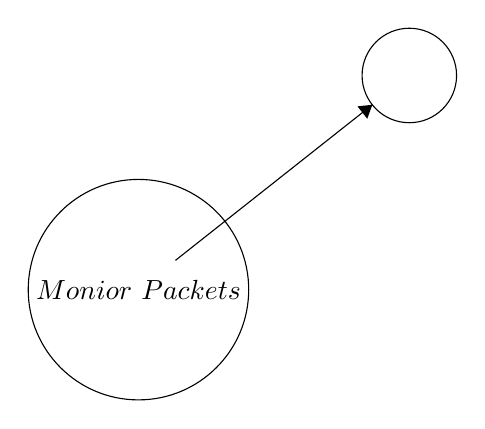
\begin{tikzpicture}[scale=0.2]
\tikzstyle{every node}+=[inner sep=0pt]
\draw [black] (13.6,-37.6) circle (7);
\draw (13.6,-37.6) node {$Monior\mbox{ }Packets$};
\draw [black] (30.8,-24) circle (3);
\draw [black] (15.95,-35.74) -- (28.45,-25.86);
\fill [black] (28.45,-25.86) -- (27.51,-25.96) -- (28.13,-26.75);
\end{tikzpicture}
\end{center}




\begin{center}
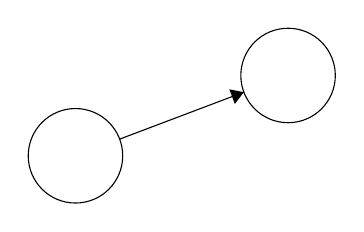
\begin{tikzpicture}[scale=0.2]
\tikzstyle{every node}+=[inner sep=0pt]
\draw [black] (16.6,-23.4) circle (3);
\draw [black] (30.1,-18.3) circle (3);
\draw [black] (19.41,-22.34) -- (27.29,-19.36);
\fill [black] (27.29,-19.36) -- (26.37,-19.18) -- (26.72,-20.11);
\end{tikzpicture}
\end{center}

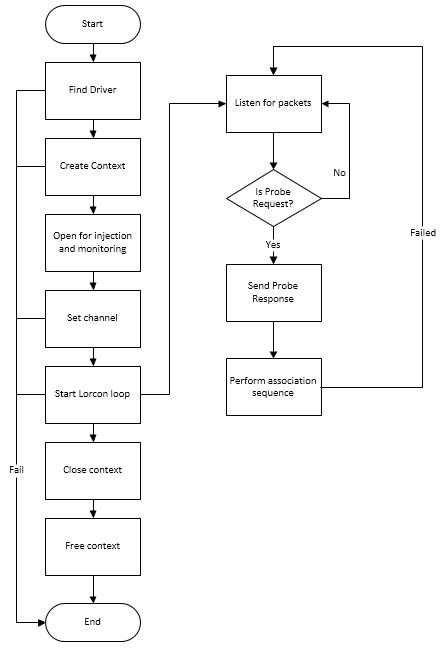
\includegraphics[width=\linewidth]{design/figures/flowchart-1.png}
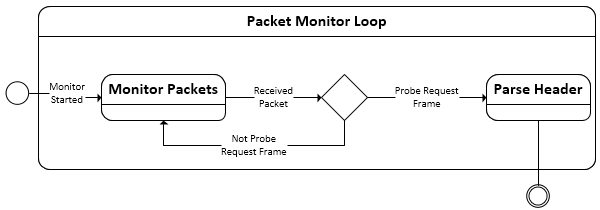
\includegraphics[width=\linewidth]{design/figures/monitorloop-umlsm.png}
\clearpage